\subsection{Fine-grained hardness under $ETH$ for \threewriter\ systems}
\label{sec:finegrained-relaxed}


\begin{lemma}\label{lem:relaxed-finegrained}
    Under ETH, there is no $2^{o(k)} \cdot n^{O(1)}$ algorithm for the consistency testing  problem for $\rlxmm$ where $k$ is the number of threads, and $n$ the number of events, even when the executions graphs are \threewriter~ and the number of writes per variable is four. 
\end{lemma}


Let $\varphi=\{C_i\}_{i \in [m]}$ be a Boolean formula over $k$ variables 
$\{x_j\}_{j \in [k]}$ and $m$ clauses of the form $C_j=(\ell_j^1, \ell_j^2, \ell_j^3)$ with where each literal is either a variable $x_i$ or its negation $\neg x_i$. 
Given a 3-CNF-SAT formula $\varphi$ with $k$ variables and $m$ clauses, we construct an abstract execution $\expartial=(\E, \po)$ with $2k+3$ threads, accessing $k+m$ memory locations $v_1, v_2, \dots, v_k, c_1, \dots, c_m$ and 2 values $1, 0$ such that $\varphi$ is satisfiable iff $\expartial_\varphi \models \rlxmm$. 
$\expartial_\varphi$ follows the general scheme depicted in Table \ref{tab:reduction-threads-relaxed}.

We remark that an $\mo$ edge from $\wt(v_i, 0)$ to $\wt(v_i,1)$ encode variable $x_i$ being set to \emph{true}, and an $\mo$ edge in the opposite direction $x_i$ being set to \emph{false}. 


\begin{wrapfigure}{r}{0.5\textwidth}
  \vspace{-\baselineskip}
  \centering
  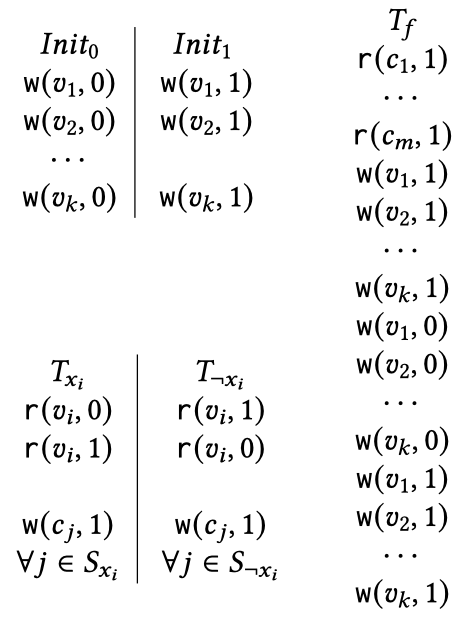
\includegraphics[width=0.3\textwidth]{Figures/relaxed-gadget.png}
    \caption{Threads in the reduction for $\rlxmm$}
    \label{tab:reduction-threads-relaxed}
\vspace{-\baselineskip}
\end{wrapfigure}
The threads $\mathsf{Init}{1}$ and $\mathsf{Init}{0}$ initialize the valuation used to evaluate the formula. For each variable $x_i$ corresponding to the Boolean variables of $\varphi$, $\mathsf{Init}{1}$ writes $1$ and $\mathsf{Init}{0}$ writes $0$. 
$T_{x_i}$ has a read statement $\rd(v_i,0)$ followed by $\rd(v_i,1)$ (which denotes reading \emph{true} for $x_i$) and sets all clauses containing $x_i$ to true, using the statement $\wt(c_j, 1)$ for all $j \in S_{x_i}$. 


Similarly, thread $T_{\neg x_i}$ reads $\rd(v_i, 1)$ followed by $\rd(v_i, 0)$ (denoting the value \emph{false} for $x_i$) and sets all clauses containing $\neg x_i$ to true. 
Finally the thread $T_{f}$ needs to make sure that all clauses are set to true, accomplished by the read statements $\rd(c_1, 1), \dots, \rd(c_m, 1)$.
Then, $T_{f}$ proceeds through the following steps (1) all the variables $v_i$s are set to $0$, followed by (2) setting all the variables $v_i$s to $1$, and finally (3) setting all the variables $v_i$s to $0$ again.
This sequence ensures that any threads $T_{x_i}$, $T_{\neg x_i}$ which were not executed in Phase 2 now have their conditions satisfied and can complete their execution. 




\begin{lemma}
    $\varphi$ is satisfiable iff $\expartial_\varphi  \models \rlxmm$.
\end{lemma}

\begin{proof}
    Suppose $A$ is a satisfying assignment for $\varphi$. We explictly describe the $\rf$ relation and $\mo$ relation as follows. 
    
    If $A(x_i) = true$:
    \begin{itemize}[leftmargin=0.1em]
    \item $\tuple{Init_0: \wt(v_i, 0)}~\rf~\tuple{T_{x_i}: \rd(v_i, 0)}$ and $\tuple{Init_1: \wt(v_i, 1)}~\rf~\tuple{T_{x_i}: \rd(v_i, 1)}$,
    \item $\tuple{T_f: \wt(v_i, 1)}~\rf~\tuple{T_{\neg x_i}: \rd(v_i, 1)}$, and $\tuple{T_f: \wt(v_i, 0)}~\rf~\tuple{T_{\neg x_i}: \rd(v_i, 0)}$. 
    \end{itemize} 
    Else, when $A(x_i) = false$, 
    \begin{itemize}[leftmargin=0.1em]
    \item $\tuple{Init_1: \wt(v_i, 1)}~\rf~\tuple{T_{\neg x_i}: \rd(v_i, 1)}$, and $\tuple{Init_0: \wt(v_i, 0)}~\rf~\tuple{T_{\neg x_i}: \rd(v_i, 0)}$,
    \item $\tuple{T_f: \wt(v_i, 0)}~\rf~\tuple{T_{ x_i}: \rd(v_i, 0)}$, and $\tuple{T_f: \wt(v_i, 1)}~\rf~\tuple{T_{ x_i}: \rd(v_i, 1)}$. 
    \end{itemize} 
            
    Coming to variables $c_i$s, for each $T_f: \rd(c_j, 1)$ there is a literal $\ell_j$ in clause $C_j$ that is true. Let $\tuple{T_{\ell_j}: \wt(c_j, 1)}~\rf~ \tuple{T_f: \rd(c_j, 1)}$. Observe that the constructed $\rf$ satisfies $\po-\rf$-acyclicity.
    
    The $\rf$ induces the following $\mo$ relation. If $A(x_i) = true$: 
    \begin{itemize}[leftmargin=0.1em]
    \item $\tuple{Init_0: \wt(v_i, 0)} ~\mo~\tuple{Init_1: \wt(v_i, 1)} ~\mo~\tuple{T_f: \wt(v_i, 1)}~\mo~\tuple{T_f: \wt(v_i, 0)} ~\mo~\\ \tuple{T_f: \wt(v_i, 1)}$
    \item For each clause $C_j$ there are three threads writing $\wt(c_j, 1)$.  For $C_j$, choose a specific literal $\ell_j$ that is made true by the satisfying assignment $A$. 
    The $\mo$ relation orders the write statements $\wt(c_j, 1)$ in literals that are set to true before $T_{\ell_j}: \wt(c_j, 1)$, and those in literals that set to false after $T_{\ell_j}: \wt(c_j, 1)$.
    \end{itemize}  
    When $A(x_i) = false$, an $\mo$ order can be defined analogously. 

    \paragraph*{Relaxed Write-coherence.} From our construction, it is easy to see $\irr(\mo_x; \po)$.

    \paragraph*{Relaxed Read-coherence.} We need to prove  $\irr(\rf^{-1}; \mo_x; \rf^{?}; \po)$. 
    If relaxed read coherence is violated, the violating pattern is of the following form there are read events $r_1$ and $r_2$, and two write events $w_1, w_2$ such that $w_1~\rf~r_1$, $w_2~\rf~r_2$, $w_1~\mo~w_2$ and $r_2~\po~r_1$.
    Such a violation can potentially happen on variables which have multiple read events in the same thread, which is only the case for $v_i$.
    We consider the various possibilities below. 
    We consider the case $A(x_i) = true$ below. 
        \begin{itemize}[leftmargin=0.1em]
            \item $\tuple{T_{x_i}: \rd(v_i, 0)} \po \tuple{T_{x_i}: \rd(v_i, 1)}$, reads-from $Init_0$ and $Init_1$ respectively, where $\mo$ agrees with the $\po$.
            \item $\tuple{T_{\neg x_i}: \rd(v_i, 1)} \po \tuple{T_{\neg x_i}: \rd(v_i, 0)}$, reads-from the first two writes on $v_i$ in $T_f$ respectively, where, once again $\mo$ agrees with the $\po$, and irreflexivity is ensured.
        \end{itemize}
        A similar argument can be made for the case the case $A(x_i) = false$.

    This shows that the constructed $\rf$ and $\mo$ are consistent with $\rlxmm$. 
    
    Conversely, suppose $\expartial_\varphi \models \rlxmm$. 
    We need to show that there are no two $\rd(c_j, 1)$ and $\rd(c_\ell, 1)$ reading from some $T_{x_i}$ and $T_{\neg x_i}$.
    Suppose not. 
    Let $\rd(c_j, 1)$ read from $T_{x_i}: \wt(c_j, 1)$ and $\rd(c_\ell, 1)$ read from $T_{\neg x_i}: \wt(c_\ell, 1)$.    
    Consider the thread $T_{x_i}$. Since $T_{x_i}: \wt(c_j, 1)$ has been read from, this means that the preceding read instructions of $T_{x_i}$ have been executed, and the only possible read from relation is as follows: 
    $\tuple{Init_0: \wt(v_i, 0)}~\rf~\tuple{T_{x_i}: \rd(v_i, 0)}$,
    and $\tuple{Init_1: \wt(v_i, 1)}~\rf~\tuple{T_{x_i}: \rd(v_i, 1)}$. 
    By relaxed read coherence axiom, this implies $\tuple{Init_0: \wt(v_i, 0)} ~\mo~\tuple{Init_1: \wt(v_i, 1)}$    

    Now, consider the thread $T_{\neg x_i}$. As argued fro $T_{x_i}$, since the last instruction has been read from, the preceding read instructions of $T_{x_i}$ have been executed with the only reads-from relation being 
    $\tuple{Init_1: \wt(v_i, 1)}~\rf~\tuple{T_{\neg x_i}: \rd(v_i, 1)}$ and $\tuple{Init_0: \wt(v_i, 0)}~\rf~\tuple{T_{\neg x_i}: \rd(v_i, 0)}$. 
    However, this violates relaxed read coherence axiom, as $\tuple{Init_0: \wt(v_i, 0)} ~\mo~\tuple{Init_1: \wt(v_i, 1)}$ but $\tuple{T_{\neg x_i}: \rd(v_i, 1)}~\po~\\ \tuple{T_{\neg x_i}: \rd(v_i, 0)}$. 
    This contradicts our assumption that there are two $\rd(c_j, 1)$ and $\rd(c_\ell, 1)$ reading from some $T_{x_i}$ and $T_{\neg x_i}$. 
    Thus, the assignment induced by the $T_i^b$ threads executed before $T_f$ satisfies $\varphi$.
\end{proof}

